\documentclass{article}

\usepackage[margin=1in]{geometry}
\usepackage{wrapfig}
\usepackage{tkz-euclide}
\usepackage{csquotes}
\usepackage{hyperref}
\usepackage{graphicx}
\usepackage{siunitx}
\usepackage{enumitem}

\title{2021 Castro Valley Junior Math Tournament \\ Middle School Division Problems}
\author{}
\date{}

\begin{document}
\maketitle

\section*{Important Information}
\textbf{Read the tournament details (\url{https://cvhsmath.weebly.com/tournament-details.html}) and the rules (\url{https://cvhsmath.weebly.com/tournament-rules.html}) before you begin.
Unless otherwise specified, answers do not need to be simplified, but they must be exact.
Unless otherwise specified, diagrams are not necessarily drawn to scale.
Submissions are due at midnight on January 30th.
Send questions to \href{mailto:cvmualphatheta@gmail.com}{\texttt{cvmualphatheta@gmail.com}}.}

\section{Moodern Art}
\begin{wrapfigure}{r}{0.35\linewidth}
	\vspace{-20pt}
	\centering
	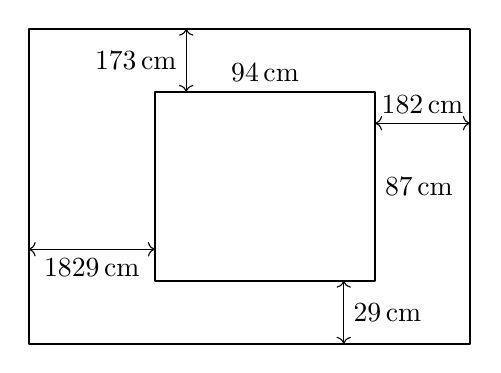
\begin{tikzpicture}[scale=0.8]
		\tkzDefPoint(0,0){A}
		\tkzDefPoint(0,5){B}
		\tkzDefPoint(7,5){C}
		\tkzDefPoint(7,0){D}
		\tkzDrawPolygon[thick](A,B,C,D)

		\tkzDefPoint(2,1){E}
		\tkzDefPoint(2,4){F}
		\tkzDefPoint(5.5,4){G}
		\tkzDefPoint(5.5,1){H}
		\tkzDrawPolygon[thick](E,F,G,H)
		\tkzLabelSegment[above](F,G){$\SI{94}{cm}$}
		\tkzLabelSegment[right](G,H){$\SI{87}{cm}$}

		\tkzDefPoint(0,1){I}
		\tkzDefPoint(2,5){J}
		\tkzDefPoint(7,4){K}
		\tkzDefPoint(5.5,0){L}
		\tkzDrawSegment[thin,arrows=<->]([yshift=0.5cm]E,[yshift=0.5cm]I)
		\tkzLabelSegment[below]([yshift=0.5cm]E,[yshift=0.5cm]I){$\SI{1829}{cm}$}
		\tkzDrawSegment[thin,arrows=<->]([xshift=0.5cm]F,[xshift=0.5cm]J)
		\tkzLabelSegment[left]([xshift=0.5cm]F,[xshift=0.5cm]J){$\SI{173}{cm}$}
		\tkzDrawSegment[thin,arrows=<->]([yshift=-0.5cm]G,[yshift=-0.5cm]K)
		\tkzLabelSegment[above]([yshift=-0.5cm]G,[yshift=-0.5cm]K){$\SI{182}{cm}$}
		\tkzDrawSegment[thin,arrows=<->]([xshift=-0.5cm]H,[xshift=-0.5cm]L)
		\tkzLabelSegment[right]([xshift=-0.5cm]H,[xshift=-0.5cm]L){$\SI{29}{cm}$}
	\end{tikzpicture}
	\vspace{-20pt}
\end{wrapfigure}
Bessie the Cow created a new painting.
It is in the shape of a rectangle $87$ centimeters tall and $94$ centimeters wide.
She hangs it on a rectangular wall such that the top edge of the painting is $173$ centimeters away from the top edge of the wall, the left edge of the painting is $1829$ centimeters away from the left edge of the wall, the right edge of the painting is $182$ centimeters away from the right edge of the wall, and the bottom edge of the painting is $29$ centimeters away from the bottom edge of the wall.
What is the area of the part of the wall that is not covered by the painting?

\section{Revomootion}
Farmer John's cows are planning a revolution to overthrow him!
The $42$ cows plan to distribute themselves among $6$ pastures.
To make sure Farmer John doesn't get suspicious, there must be at least two cows in each pasture, each pasture must have a different number of cows, and no pasture can have exactly $3$ or $5$ cows.
To help the cows calculate their chance of succeeding, find the greatest number of cows that can be in any one pasture.

\section{On the Moove}
Bessie the Cow and her sister Bailey the Cow leave their barn at the same time, running at a constant speed on a narrow and straight road.
Bessie went northbound traveling at $42$ miles per hour.
After $2$ hours, Bailey is $30$ miles south of Bessie.
What was Bailey's speed in miles per hour and which direction was she traveling in?

\section{Cowld}
\begin{wrapfigure}{r}{0.3\linewidth}
    \vspace{-50pt}
    \centering
	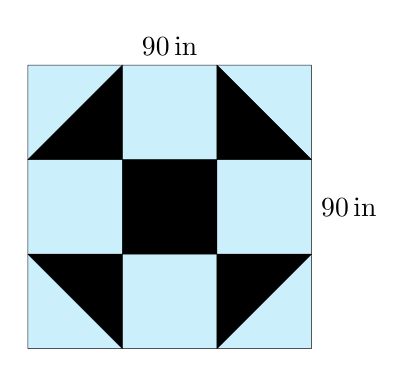
\begin{tikzpicture}[scale=0.4]
		\tkzDefPoint(0,0){A}
		\tkzDefPoint(9,0){B}
		\tkzDefSquare(A,B)
		\tkzGetPoints{C}{D}
		\tkzDrawPolygon[fill=cyan!20](A,B,C,D)
		\tkzLabelSegment[above](C,D){$\SI{90}{in}$}
		\tkzLabelSegment[right](B,C){$\SI{90}{in}$}

		\tkzDefPoint(3,3){E}
		\tkzDefPoint(6,3){F}
		\tkzDefSquare(E,F)
		\tkzGetPoints{G}{H}
		\tkzDrawPolygon[fill=black](E,F,G,H)
		
		\tkzDefPoint(3,0){I}
		\tkzDefPoint(6,0){J}
		\tkzDefPoint(9,3){K}
		\tkzDefPoint(9,6){L}
		\tkzDefPoint(6,9){M}
		\tkzDefPoint(3,9){N}
		\tkzDefPoint(0,6){O}
		\tkzDefPoint(0,3){P}
		\tkzDrawPolygon[fill=black](E,I,P)
		\tkzDrawPolygon[fill=black](F,J,K)
		\tkzDrawPolygon[fill=black](G,L,M)
		\tkzDrawPolygon[fill=black](H,N,O)
	\end{tikzpicture}
	\vspace{-20pt}
\end{wrapfigure}
Cowboy Alex wants to make a giant blanket for his cows with a specific pattern because they are cold.
If the blanket uses the pattern $36$ times and one side of the pattern is $90$ inches long, how many square inches of black fabric will he need to make the blanket? This diagram is drawn to scale. Each of the small squares in the pattern is \SI{30}{in} by \SI{30}{in}.

\section{Cownt the Rectangles}
\begin{wrapfigure}{r}{0.35\linewidth}
	\vspace{-20pt}
	\centering
	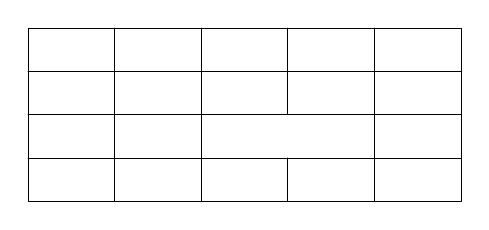
\begin{tikzpicture}[scale=0.55]
		\tkzDefPoint(0,0){A}
		\tkzDefPoint(0,4){B}
		\tkzDefPoint(10,4){C}
		\tkzDefPoint(10,0){D}
		\tkzDrawPolygon(A,B,C,D)

		\tkzDefPoint(0,1){E}
		\tkzDrawSegment(E,[xshift=10cm]E)
		\tkzDefPoint(0,2){F}
		\tkzDrawSegment(F,[xshift=10cm]F)
		\tkzDefPoint(0,3){G}
		\tkzDrawSegment(G,[xshift=10cm]G)

		\tkzDefPoint(2,0){H}
		\tkzDrawSegment(H,[yshift=4cm]H)
		\tkzDefPoint(4,0){I}
		\tkzDrawSegment(I,[yshift=4cm]I)
		\tkzDefPoint(6,0){J}
		\tkzDrawSegment(J,[yshift=1cm]J)
		\tkzDrawSegment([yshift=2cm]J,[yshift=4cm]J)
		\tkzDefPoint(8,0){K}
		\tkzDrawSegment(K,[yshift=4cm]K)
	\end{tikzpicture}
	\vspace{-20pt}
\end{wrapfigure}
Bessie the Cow found a piece of paper with the following figure printed on it.
She wants to know how many rectangles are in the figure.
Help her by finding the number of rectangles of any size that is in this figure, including rectangles which contain multiple smaller rectangles.

\section{Soccow}
Rancher Cedric decided to hold a soccow tournament for his cows.
Bessie the Cow's team, the Tactful Tauruses, lost $8$ of their first $10$ games.
If they will play $30$ more games in this tournament, how many of the remaining games do they need to win in order to make the total number of games which they won at least twice as much as the total number of games which they lost?

\section{Green Cows 1}
Help Bessie the Cow answer the question ``How much grass can a green cow chow if green cows can chow grass?''
Bessie and Elsie both chow grass at constant rates.
If Bessie can chow all the grass in a field in $3$ hours and Elsie can chow all the grass in the same field in $4$ minutes, how long will it take for them to chow all the grass in this field together?
Your answer must be exact.

\section{Green Cows 2}
Bessie the Cow still hasn't figured out how much grass a green cow can chow if green cows can chow grass.
If $5$ green cows can chow $8$ square meters of grass in $20$ minutes, how many green cows are needed to chow $10$ square meters of grass in at most $15$ minutes?
Assume that all green cows in this problem chow grass at the same constant rate.

\section{Moogic}
\begin{wrapfigure}{r}{0.35\linewidth}
	\vspace{-20pt}
	\centering
	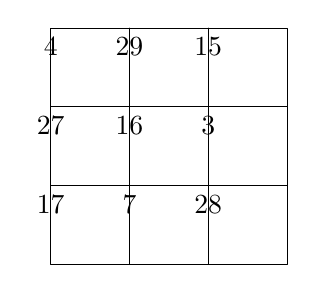
\begin{tikzpicture}
		\tkzDefPoint(0,0){A}
		\tkzDefPoint(3,0){B}
		\tkzDefSquare(A,B)
		\tkzGetPoints{C}{D}
		\tkzDrawPolygon(A,B,C,D)

		\tkzDefPoint(1,3){E}
		\tkzDefPoint(2,3){F}
		\tkzDrawSegment(E,[yshift=-3cm]E)
		\tkzDrawSegment(F,[yshift=-3cm]F)

		\tkzDefPoint(0,2){G}
		\tkzDefPoint(0,1){H}
		\tkzDrawSegment(G,[xshift=3cm]G)
		\tkzDrawSegment(H,[xshift=3cm]H)

		\tkzDefPoint(1,2){J}
		\tkzDefPoint(2,2){K}
		\tkzDefPoint(1,1){L}
		\tkzDefPoint(2,1){M}

		\foreach \name\value in {D/$4$, E/$29$, F/$15$, G/$27$, J/$16$, K/$3$, H/$17$, L/$7$, M/$28$}
		{
			\tkzLabelPoint(\name){\value}
		}


	\end{tikzpicture}
	\vspace{-10pt}
\end{wrapfigure}
Bessie the Cow wanted to learn how to do magic, but she got distracted on the internet and ended up learning about magic squares.
In a magic square, the sum of the numbers in each row, each column, and the two diagonals are the same.
(One diagonal contains the numbers $4$, $16$, and $28$, while the other contains $17$, $16$, and $15$.)
If exactly two numbers are changed in this grid, the result is a magic square.
Which two numbers must be changed and what values should they be changed to?

\section{Mooish}
Farmer Paul has two types of cows: truthy cows and falsy cows.
Physically, they are indistinguishable.
They all speak mooish, and they can be distinguished by how they answer questions.
The truthy cows always reply truthfully, and the falsy cows always lie.
Bessie the Cow had a conversation with three of Farmer Paul's cows: Annabelle, Bossy, and Cornelius.
Here's a translation of the conversation.
\begin{displayquote}
    Bessie: Are any of you falsy? \\
    Annabelle: At least one of us is falsy. \\
    Bessie: Are Bossy and Cornelius both truthy? \\
    Bossy: Yes. \\
    Bessie: Are Annabelle and Bossy both truthy? \\
    Cornelius: No.
\end{displayquote}
What is the type of each cow?

\section{Cowkies}
When Bessie the Cow was visiting a nearby farm, she noticed that there is a large group of cows.
She brought some cookies to make new cow friends, but she didn't know how many cows there were in the group!
She counted a total of $87$ black spots and $83$ white spots, not including her own spots.
Each cow either has two black spots and three white spots or three black spots and two white spots.
How many cows are in the group, not including Bessie?

\section{Moorio Kart}
Cowboy Alex gave Bessie the Cow a new racing game called Moorio Kart!
She let all of her cow friends play, and then asked each cow whether they liked each of the three courses.
$86$ cows said they liked Bowser Cowstle, $25$ cows said they liked Cowconut Mall, and $67$ cows said they liked Moo Moo Meadows.
Some cows might have liked two courses, and no cow liked all three courses.
What is the fewest possible number of friends which Bessie could have had?

\section{Moo York Bagels}
Bessie the Cow now lives in Moo York and every day she buys a bagel from Billie the Bagel Cow.
The type of bagel that she buys depends on her mood.
If Bessie is happy, she will spend $\$1000$ on a toasted blueberry bagel.
If Bessie is sad, she will spend $\$620$ on a strawberry cream cheese bagel.
On any given day Bessie has a $68\%$ chance of being happy.
On average, how much does Bessie spend on the bagels each day?
Round your answer to the nearest cent.

\section{Mooilk}
Farmer Julia wants to measure out exactly $25.5$ gallons of milk in a large storage bin. 
The bin is initially empty. 
Farmer Julia has a $2$ gallon bucket and a $3.5$ gallon bucket. 
In one move, she can add $2$ gallons of milk to the bin or add $3.5$ gallons of milk to the bin. 
If there is at least $5$ gallons of milk in the bin, she can also remove $2$ gallons of milk or remove $3.5$ gallons of milk in one move. 
What is the least possible number of moves needed to end with exactly $25.5$ gallons of milk in the bin? 

\section{Mooving Cow}
Bessie the Cow is $5$ meters north of Farmer Pearson's house.
She starts running east at $2$ meters per second.
After how many seconds will she be exactly $10$ meters away from Farmer Pearson's house?
Your answer must be exact.

\section{Moss-cow}
Bessie the Cow is currently staying in London during a world tour to find the tastiest grass.
She prepares to visit Moscow next.
The route from London to Moscow is $1600$ miles long.
First, Bessie will ride a plane flying from London to Warsaw traveling at $560$ miles per hour.
Then, she will ride a train moving at $60$ miles per hour.
If the whole journey took $19.5$ hours, how many minutes did Bessie spend on the plane?
Round your answer to the nearest integer.
Assume that the time it takes for Bessie to transfer from the plane to the train is negligible.

\section{Look Mom No Proof!}
Bessie the Cow found a website called \url{https://vixra.org/} which mostly publishes scientific nonsense.
There's a paper (\url{https://vixra.org/abs/2008.0229}) which presents a simple method that supposedly checks whether integers greater than $5$ are prime.
It makes the following statement without proof:
\begin{displayquote}
    The answer to whether the given numbers are prime numbers is to check that:
    \begin{enumerate}[label=\alph*)]
        \item The numbers are not even numbers (the last digit is not divisible by $2$);
        \item The last digit of numbers in not $5$;
        \item The sum of the digits of each of the remaining numbers is not divisible by $3$.
    \end{enumerate}
    A number that meets the above criteria is either a prime or a power [of a] prime.
\end{displayquote}
Find the smallest counterexample that disproves this claim.

\section{Completely Organic Watermelons (C.O.W.)}
Bessie the Cow was looking through the Barnyard Bazaar for some fresh produce when she spotted some Completely Organic Watermelons!
Bella the Watermelon Cow has $18$ \emph{different} watermelons for sale: $5$ are large, $6$ are medium, and $7$ are small.
Bessie wants to buy three watermelons that aren't all the same size.
(In other words, she wants to buy three watermelons of at least two different sizes.)
In how many ways can this be done?
The order in which she buys them doesn't matter, but each watermelon is unique and different from other watermelons of the same size.

\section{Cowtapult}
\begin{wrapfigure}{r}{0.35\linewidth}
    \vspace{-30pt}
    \centering
    \includegraphics[scale=0.4]{cowtapult.png}
    \vspace{-30pt}
\end{wrapfigure}
Cowboy Alex's barn is being attacked!!!!!
The enemy cows are in a cart that's currently $80$ meters north and $50$ meters east of the barn, and it is traveling west at $10$ meters per second.
Bessie the Cow is operating a cowtapult that is $15$ meters north of the barn.
The cowtapult launches a hay bale with a horizontal speed of $20$ meters per second in a direction that is $30$ degrees west from north.
Bessie wants to hit the enemy cart using the cowtapult.
When should she launch the hay bale?
Express your answer as a decimal in seconds, rounded to three digits after the decimal point.

\section{woC}
Bessie the Cow chooses an integer randomly and uniformly from $1000$ to $8375$ inclusive, reverses the digits, then discards any leading zeros.
What is the expected value of the result?
Your answer must be exact.

\section{Baa Baa Bazaar}
\begin{wrapfigure}{r}{0.5\linewidth}
	\vspace{-20pt}
	\centering
	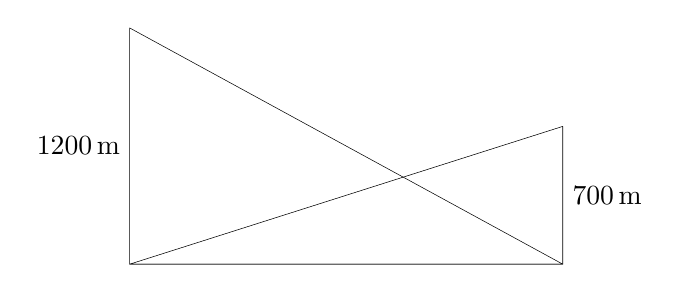
\begin{tikzpicture}[scale=0.25]
		\tkzDefPoint(0,0){A}
		\tkzDefPoint(0,12){B}
		\tkzDefPoint(22,0){C}
		\tkzDefPoint(22,7){D}
		\tkzDrawPolygon(A,B,C)
		\tkzDrawPolygon(A,C,D)
		\tkzLabelSegment[left](A,B){\SI{1200}{m}}
		\tkzLabelSegment[right](C,D){\SI{700}{m}}
	\vspace{-20pt}
	\end{tikzpicture}
\end{wrapfigure}
Bessie the Cow wants to visit the famous Baa Baa Bazaar, but the sheep have set it up in a great canyon with vertical cliffs on both sides.
One cliff is $700$ meters high, while the other is $1200$ meters high.
A perfectly straight zip line runs from the foot of each cliff to the top of the other cliff.
At what height above the ground do the two cables meet?

\section{The Great Cow Chase}
Oh no! Kiran the Cow is making an escape!
Kiran is $10$ miles south of Farmer John, and he starts running east at $15$ miles per hour.
Farmer John can move at $30$ miles per hour.
How long will it take for Farmer John to catch Kiran if Farmer John uses the fastest possible strategy?
Express your answer in seconds, rounded to the nearest integer.

\section{Rowdy Cow}
After Rancher Cedric caught Kiran the Cow in the Great Cow Chase, Kiran decided to trample the grass and terrorize the chickens.
Rancher Cedric had enough, and he decided to lock him in a pen.
The pen is in the shape of an equilateral triangle, and each side is $500$ meters long.
The rowdy cow is tied to one corner, so that the portion of the field it can reach is exactly half of the total area.
If Kiran and the rope both have zero width, how long is the rope in meters?
Express your answer as a decimal rounded to two digits after the decimal point.

\section{My Cow Ate My Homework}
Bessie the Cow obtained Chloe's math homework again.
While she was enjoying this tasty snack, she noticed one problem that seemed very interesting.
Here's the problem statement:
\begin{displayquote}
	If two real numbers $a$ and $b$ are generated randomly and uniformly such that $-9 < a < 9$ and $-9 < b < 9$, what is the probability that $(a + b)^2 \leq 2ab + 9$?
	Your answer must be exact.
\end{displayquote}
Bessie is bad at math, so help her by solving this problem.

\section{Cowloring}
\begin{wrapfigure}{r}{0.35\linewidth}
    \vspace{-20pt}
    \centering
    \includegraphics[scale=0.35]{cowloring.png}
    \vspace{-20pt}
\end{wrapfigure}
Bessie the Cow found a piece of paper with this figure printed on it and she wants to color it using red, green, and/or blue.
In how many ways can she do this if the orientation of the figure doesn't matter?
Each region in the figure must have exactly one of the three colors.
Two coloring schemes are considered equivalent if one can be obtained by rotating the other.
\end{document}
